\documentclass[border=1pt]{standalone}
% Shared preamble for standalone figures in this directory.
% Compile with XeLaTeX from 讲义/figs, or via the figures target.
\usepackage{ctex}
\usepackage{amsmath}
\usepackage{amssymb}
\usepackage{bm}
\usepackage{mathtools}
\usepackage{tikz}
\renewcommand{\vec}[1]{\boldsymbol{#1}}
\newcommand{\cC}{\mathcal{C}}
\newcommand{\cD}{\mathcal{D}}
\newcommand{\R}{\mathbf{R}}
\usetikzlibrary{
    arrows.meta,
    calc,
    decorations.markings,
    angles,
    quotes,
    positioning,
    patterns,
    shapes.geometric
}

\begin{document}
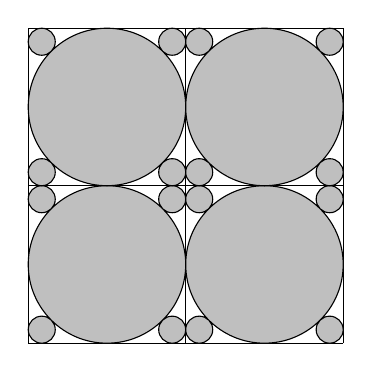
\begin{tikzpicture}[scale=2]
    \draw (0, 0) grid (2, 2);
    \foreach \i in {0.5, 1.5}
        \foreach \j in {0.5, 1.5}
            \draw[fill=gray!50] (\i, \j) circle (0.5)
                \foreach \k in {45, 135, 225, 315} {($(\i, \j) + (\k:{sqrt(2)/(sqrt(2)+1)})$) circle ({(sqrt(2)-1)/(2+2*sqrt(2))})};
\end{tikzpicture}

\end{document}
